\noindent\rule{\linewidth}{0.6pt}\\

\section{\large \textcolor{blue}{As leis de conservação na Mecânica Clássica}}

\begin{flushleft}
\textbf{\textcolor{blue}{\Large Quest\~ao - Medidor de Vazão (Tubo de Venturi)}}\\
\noindent

\subsection{Quest\~ao - Medidor de Vazão (Tubo de Venturi)}

Um fluido incompressível e não viscoso escoa horizontalmente através de um tubo de Venturi. O tubo possui uma seção larga de área \( A_1 \) e uma seção estreita de área \( A_2 \), com \( A_1 > A_2 \). Dois tubos manométricos estão conectados nas duas seções, e observa-se um desnível \( h \) entre os níveis do fluido nesses tubos.

Sabendo que a diferença de altura nos tubos manométricos é devida à diferença de pressão entre as seções do tubo, determine a expressão para a velocidade do fluido \( v_1 \) na seção de maior área \( A_1 \), em função de \( g \), \( h \), \( A_1 \) e \( A_2 \).



\begin{itemize}
\item[(A)] \( v_1 = \sqrt{ \dfrac{2gh}{1 - \left( \dfrac{A_2}{A_1} \right)^2} } \)
\item[(B)] \( v_1 = \sqrt{ \dfrac{gh}{\left( \dfrac{A_1}{A_2} \right)^2 - 1} } \)
\item[(C)] \( v_1 = \sqrt{ \dfrac{2gh}{\left( \dfrac{A_1}{A_2} \right)^2 - 1} } \)
\item[(D)] \( v_1 = \dfrac{A_2}{A_1} \sqrt{ 2gh } \)
\item[(E)] \( v_1 = \sqrt{ 2gh \left( \dfrac{A_2}{A_1} \right)^2 } \)
\end{itemize}

\vspace{0.5cm}

\textcolor{red}{\textbf{Solução:}}\\

Pelo teorema de Bernoulli (sem variação de altura) e pela equação da continuidade, temos:

\[
P_1 - P_2 = \frac{\rho}{2}(v_2^2 - v_1^2) \quad \text{e} \quad v_2 = \frac{A_1}{A_2} v_1
\]

Substituindo:

\[
\rho g h = \frac{\rho}{2} \left[ \left( \frac{A_1}{A_2} \right)^2 v_1^2 - v_1^2 \right]
\Rightarrow 2gh = v_1^2 \left[ \left( \frac{A_1}{A_2} \right)^2 - 1 \right]
\]

\[
\Rightarrow v_1 = \sqrt{ \frac{2gh}{\left( \dfrac{A_1}{A_2} \right)^2 - 1} }
\]

A resposta correta é alternativa \colorbox{green!50}{\textbf{(C)}}.

\end{flushleft}

\begin{flushleft}
\textbf{\textcolor{blue}{\Large Quest\~ao 23}}\\
\subsection{Quest\~ao 23 - Quantidade de Momento Linear}
Uma bola de aço de \(2\,\text{kg}\) se desloca horizontalmente a \(10\,\text{m/s}\) sobre uma 
superfície sem atrito e colide frontalmente com uma segunda bola de \(3\,\text{kg}\), que se move 
no mesmo sentido a \(4\,\text{m/s}\). A colisão entre as bolas é perfeitamente elástica. Com base nessas 
informações, qual será a velocidade da bola de \(2\,\text{kg}\) após a colisão?


\begin{itemize}
\item[(A)] -2 m/s.
\item[(B)]  2 m/s.
\item[(C)]  2,8 m/s.
\item[(D)]  8,8 m/s.
\item[(E)]  10 m/s.
\end{itemize}

\vspace{0.5cm}

\begin{center}
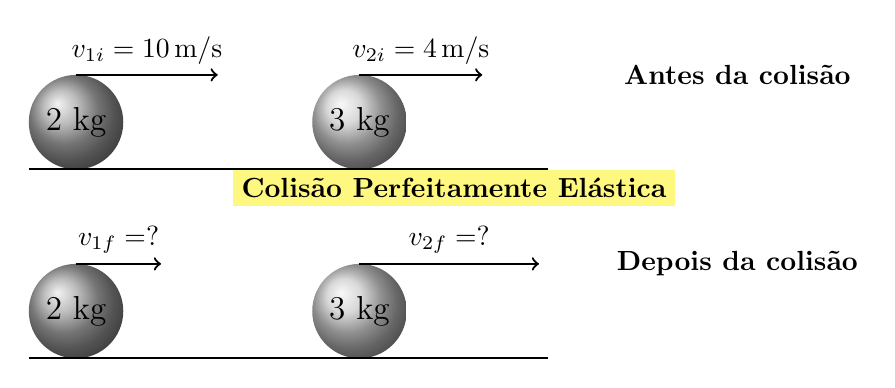
\begin{tikzpicture}[scale=1.2]

% Antes da colisão
\node at (7,2.5) {\textbf{Antes da colisão}};
% Bola 1
\shade[ball color=gray!70] (0,2) circle (0.5);
\node at (0,2) {\large 2 kg};
% Velocidade bola 1
\draw[->, thick] (0,2.5) -- (1.5,2.5) node[midway, above] {\(v_{1i}=10\,\mathrm{m/s}\)};

% Bola 2
\shade[ball color=gray!40] (3,2) circle (0.5);
\node at (3,2) {\large 3 kg};
% Velocidade bola 2
\draw[->, thick] (3,2.5) -- (4.3,2.5) node[midway, above] {\(v_{2i}=4\,\mathrm{m/s}\)};

\node at (4,1.3) {\colorbox{yellow!50}{\textbf{Colisão Perfeitamente Elástica}}};
% Linha base
\draw[thick] (-0.5,1.5) -- (5,1.5);

% Depois da colisão
\node at (7,0.5) {\textbf{Depois da colisão}};
% Bola 1
\shade[ball color=gray!70] (0,0) circle (0.5);
\node at (0,0) {\large 2 kg};
% Velocidade bola 1 final
\draw[->, thick] (0,0.5) -- (0.9,0.5) node[midway, above] {\(v_{1f}=?\)};

% Bola 2
\shade[ball color=gray!40] (3,0) circle (0.5);
\node at (3,0) {\large 3 kg};
% Velocidade bola 2 final
\draw[->, thick] (3,0.5) -- (4.9,0.5) node[midway, above] {\(v_{2f}=?\)};

% Linha base
\draw[thick] (-0.5,-0.5) -- (5,-0.5);

\end{tikzpicture}
\end{center}

\textcolor{red}{\textbf{Solução:}}\\

\begin{itemize}
    \item Massa da primeira bola: \(m_1 = 2\,\text{kg}\)
    \item Velocidade inicial da primeira bola: \(v_{1i} = 10\,\text{m/s}\)
    \item Massa da segunda bola: \(m_2 = 3\,\text{kg}\)
    \item Velocidade inicial da segunda bola: \(v_{2i} = 4\,\text{m/s}\)
\end{itemize}

Uma colisão perfeitamente elástica obedece simultaneamente à:

\begin{itemize}
    \item \textbf{Conservação da quantidade de movimento:}
    \[
        \sum Q_{i} = \sum Q_{f}
    \]
    
    \[
    m_1v_{1i} + m_2v_{2i} = m_1v_{1f} + m_2v_{2f}
    \]
    \item \textbf{Conservação da energia cinética:}
    \[
    \frac{1}{2}m_1v_{1i}^2 + \frac{1}{2}m_2v_{2i}^2 = \frac{1}{2}m_1v_{1f}^2 + \frac{1}{2}m_2v_{2f}^2
    \]
\end{itemize}

Onde:
\begin{itemize}
    \item \(v_{1i}\) e \(v_{2i}\): velocidades iniciais das massas \(m_1\) e \(m_2\)
    \item \(v_{1f}\) e \(v_{2f}\): velocidades finais das massas \(m_1\) e \(m_2\)
\end{itemize}

\subsection*{Dedução da Fórmula Direta}

Para facilitar a resolução sem precisar resolver um sistema de duas equações, aplicamos uma transformação clássica: a equação das velocidades relativas.
Em colisões perfeitamente elásticas em uma dimensão, podemos usar o coeficiente de restituição (\(e\)) \'e definido pela raz\~ao entre a velocidade relativas de afastamento
e aproximação:

\[
e = \frac{v_{afastamento}}{v_{aproximada\c{c}\~ao}}
\]

\[
e = \frac{v_{2f} - v_{1f}}{v_{1i} - v_{2i}} = 1
\]

\[
v_{1i} - v_{2i} = -(v_{1f} - v_{2f})
\]

Ou seja:

\[
v_{1i} - v_{2i} = v_{2f} - v_{1f}
\]

Agora temos duas equações:

\begin{equation}
m_1v_{1i} + m_2v_{2i} = m_1v_{1f} + m_2v_{2f} \tag{1}
\end{equation}

\begin{equation}
v_{1i} - v_{2i} = v_{2f} - v_{1f} \tag{2}
\end{equation}

\subsection*{Resolvendo o Sistema}

Da equação (2):

\[
\boxed{
v_{2f} = v_{1i} - v_{2i} + v_{1f}
}
\]

Substituindo isso na equação (1):

\[
m_1v_{1i} + m_2v_{2i} = m_1v_{1f} + m_2(v_{1i} - v_{2i} + v_{1f})
\]

Distribuindo:

\[
m_1v_{1i} + m_2v_{2i} = m_1v_{1f} + m_2v_{1i} - m_2v_{2i} + m_2v_{1f}
\]

Agrupando os termos:

\[
m_1v_{1i} - m_2v_{1i} + m_2v_{2i} + m_2v_{2i} = (m_1 + m_2)v_{1f}
\]

\[
(m_1 - m_2)v_{1i} + 2m_2v_{2i} = (m_1 + m_2)v_{1f}
\]

Finalmente, isolando \(v_{1f}\):

\[
\boxed{
v_{1f} = \frac{(m_1 - m_2)v_{1i} + 2m_2v_{2i}}{m_1 + m_2}
}
\]

\subsection*{Cálculo Numérico}

Substituindo os valores fornecidos:

\[
v_{1f} = \frac{(2\,\text{kg} - 3\,\text{kg}) \times 10\,\text{m/s} + 2 \times 3\,\text{kg} \times 4\,\text{m/s}}{2\,\text{kg} + 3\,\text{kg}}
\]

\[
v_{1f} = \frac{(-1)\times10 + 24}{5}
\]

\[
v_{1f} = \frac{-10 + 24}{5}
\]

\[
v_{1f} = \frac{14}{5}
\]

\[
\boxed{v_{1f} = 2{,}8\,\text{m/s}}
\]

no mesmo sentido original do movimento.

A velocidade da bola de \(2\,\text{kg}\) após a colisão será \(2{,}8\,\text{m/s}\). \textbf{Resposta: \colorbox{green!50}{(C)}}. 

\end{flushleft}

\begin{flushleft}
\textbf{\textcolor{blue}{\Large Quest\~ao 36 }}\\
\noindent
\subsection{Quest\~ao 36 - Conserva\c{c}\~ao Momento Angular}
Observe a figura a seguir.

\begin{figure}[h]
\centering
\includegraphics[width=0.8\textwidth]{figures/momento_angular.png}
\end{figure}

Uma bala de massa m se move horizontalmente com
velocidade v. A bala atinge a borda de um disco sólido, que
está inicialmente em repouso, ficando cravada nele (ver a
figura). O disco tem massa M, raio R, momento de inércia
$MR^{2}/2$ e está livre para girar em torno de seu eixo. Qual é a
velocidade angular do disco imediatamente após a bala ser
cravada nele?

\begin{itemize}
\item[(A)] $\Huge \omega = \frac{Mv}{(m+\frac{M}{2})R}$
\item[(B)] $\Huge \omega = \frac{mv}{(m+\frac{M}{2})R}$
\item[(C)] $\Huge \omega = \frac{mv}{(\frac{M}{2}-m)R}$
\item[(D)] $\Huge \omega = \frac{Mv}{(\frac{M}{2}-m)R}$
\end{itemize}

\vspace{0.5cm}

\textcolor{red}{\textbf{Solução:}}\\

\textbf{Princípio:}  
Como não há torques externos atuando em torno do eixo vertical, o momento angular do sistema em relação ao eixo é conservado.

\subsubsection*{Antes da colisão}
O momento angular do sistema em torno do eixo é apenas devido à bala:
\[
L_{\text{inicial}} = m v R
\]

\subsubsection*{Depois da colisão}
Após a colisão, a bala fica presa ao disco na borda, e o sistema (disco + bala) gira com velocidade angular \(\omega\).

Momento angular do disco:
\[
L_{\text{disco}} = I_{\text{disco}} \cdot \omega = \frac{1}{2} M R^2 \cdot \omega
\]

Momento angular da bala (considerada puntiforme a distância \(R\) do eixo):
\[
L_{\text{bala}} = m R^2 \cdot \omega
\]

Assim, o momento angular total após a colisão é:
\[
L_{\text{final}} = \left( \frac{1}{2} M R^2 + m R^2 \right) \omega
\]

\subsubsection*{Conservação do momento angular}
\[
L_{\text{inicial}} = L_{\text{final}}
\]

\[
m v R = \left( \frac{1}{2} M R^2 + m R^2 \right) \omega
\]

Dividindo ambos os lados por \(R\):
\[
m v = \left( \frac{1}{2} M + m \right) R \omega
\]

Isolando \(\omega\):
\[
\omega = \frac{m v}{R \left( \frac{1}{2} M + m \right)}
\]

\subsection*{Resposta final:}
\[
\boxed{
\omega = \frac{m v}{\left(m + \frac{1}{2} M\right)R}
}
\]

A resposta correta é alternativa \colorbox{green!50}{\textbf{B}}.
\end{flushleft}

\begin{flushleft}
\textbf{\textcolor{blue}{\Large Quest\~ao - }}\\
\noindent

\subsection{Quest\~ao }

\begin{itemize}
\item[(A)] 
\item[(B)] 
\item[(C)]
\item[(D)] 
\item[(E)] 
\end{itemize}

\vspace{0.5cm}

\textcolor{red}{\textbf{Solução:}}\\


A resposta correta é alternativa \colorbox{green!50}{\textbf{...}}.

\end{flushleft}

\noindent\rule{\linewidth}{0.6pt}\\
